% GNUPLOT: LaTeX picture with Postscript
\begingroup
  % Encoding inside the plot.  In the header of your document, this encoding
  % should to defined, e.g., by using
  % \usepackage[cp1252,<other encodings>]{inputenc}
  \inputencoding{cp1252}%
  \fontfamily{phv}%
  \selectfont
  \makeatletter
  \providecommand\color[2][]{%
    \GenericError{(gnuplot) \space\space\space\@spaces}{%
      Package color not loaded in conjunction with
      terminal option `colourtext'%
    }{See the gnuplot documentation for explanation.%
    }{Either use 'blacktext' in gnuplot or load the package
      color.sty in LaTeX.}%
    \renewcommand\color[2][]{}%
  }%
  \providecommand\includegraphics[2][]{%
    \GenericError{(gnuplot) \space\space\space\@spaces}{%
      Package graphicx or graphics not loaded%
    }{See the gnuplot documentation for explanation.%
    }{The gnuplot epslatex terminal needs graphicx.sty or graphics.sty.}%
    \renewcommand\includegraphics[2][]{}%
  }%
  \providecommand\rotatebox[2]{#2}%
  \@ifundefined{ifGPcolor}{%
    \newif\ifGPcolor
    \GPcolortrue
  }{}%
  \@ifundefined{ifGPblacktext}{%
    \newif\ifGPblacktext
    \GPblacktextfalse
  }{}%
  % define a \g@addto@macro without @ in the name:
  \let\gplgaddtomacro\g@addto@macro
  % define empty templates for all commands taking text:
  \gdef\gplbacktext{}%
  \gdef\gplfronttext{}%
  \makeatother
  \ifGPblacktext
    % no textcolor at all
    \def\colorrgb#1{}%
    \def\colorgray#1{}%
  \else
    % gray or color?
    \ifGPcolor
      \def\colorrgb#1{\color[rgb]{#1}}%
      \def\colorgray#1{\color[gray]{#1}}%
      \expandafter\def\csname LTw\endcsname{\color{white}}%
      \expandafter\def\csname LTb\endcsname{\color{black}}%
      \expandafter\def\csname LTa\endcsname{\color{black}}%
      \expandafter\def\csname LT0\endcsname{\color[rgb]{1,0,0}}%
      \expandafter\def\csname LT1\endcsname{\color[rgb]{0,1,0}}%
      \expandafter\def\csname LT2\endcsname{\color[rgb]{0,0,1}}%
      \expandafter\def\csname LT3\endcsname{\color[rgb]{1,0,1}}%
      \expandafter\def\csname LT4\endcsname{\color[rgb]{0,1,1}}%
      \expandafter\def\csname LT5\endcsname{\color[rgb]{1,1,0}}%
      \expandafter\def\csname LT6\endcsname{\color[rgb]{0,0,0}}%
      \expandafter\def\csname LT7\endcsname{\color[rgb]{1,0.3,0}}%
      \expandafter\def\csname LT8\endcsname{\color[rgb]{0.5,0.5,0.5}}%
    \else
      % gray
      \def\colorrgb#1{\color{black}}%
      \def\colorgray#1{\color[gray]{#1}}%
      \expandafter\def\csname LTw\endcsname{\color{white}}%
      \expandafter\def\csname LTb\endcsname{\color{black}}%
      \expandafter\def\csname LTa\endcsname{\color{black}}%
      \expandafter\def\csname LT0\endcsname{\color{black}}%
      \expandafter\def\csname LT1\endcsname{\color{black}}%
      \expandafter\def\csname LT2\endcsname{\color{black}}%
      \expandafter\def\csname LT3\endcsname{\color{black}}%
      \expandafter\def\csname LT4\endcsname{\color{black}}%
      \expandafter\def\csname LT5\endcsname{\color{black}}%
      \expandafter\def\csname LT6\endcsname{\color{black}}%
      \expandafter\def\csname LT7\endcsname{\color{black}}%
      \expandafter\def\csname LT8\endcsname{\color{black}}%
    \fi
  \fi
    \setlength{\unitlength}{0.0500bp}%
    \ifx\gptboxheight\undefined%
      \newlength{\gptboxheight}%
      \newlength{\gptboxwidth}%
      \newsavebox{\gptboxtext}%
    \fi%
    \setlength{\fboxrule}{0.5pt}%
    \setlength{\fboxsep}{1pt}%
\begin{picture}(15874.00,8502.00)%
    \gplgaddtomacro\gplbacktext{%
      \csname LTb\endcsname%%
      \put(1342,704){\makebox(0,0)[r]{\strut{}\textbf{\scriptsize $0$}}}%
      \csname LTb\endcsname%%
      \put(1342,7627){\makebox(0,0)[r]{\strut{}\textbf{\scriptsize $2.49$}}}%
      \csname LTb\endcsname%%
      \put(1342,2094){\makebox(0,0)[r]{\strut{}\textbf{\scriptsize $0.5$}}}%
      \csname LTb\endcsname%%
      \put(1342,3484){\makebox(0,0)[r]{\strut{}\textbf{\scriptsize $1$}}}%
      \csname LTb\endcsname%%
      \put(1342,4874){\makebox(0,0)[r]{\strut{}\textbf{\scriptsize $1.5$}}}%
      \csname LTb\endcsname%%
      \put(1342,6265){\makebox(0,0)[r]{\strut{}\textbf{\scriptsize $2$}}}%
      \csname LTb\endcsname%%
      \put(1474,484){\makebox(0,0){\strut{}\textbf{\scriptsize $0$}}}%
      \csname LTb\endcsname%%
      \put(15477,484){\makebox(0,0){\strut{}\textbf{\scriptsize $7470$}}}%
      \csname LTb\endcsname%%
      \put(2411,484){\makebox(0,0){\strut{}\textbf{\scriptsize $500$}}}%
      \csname LTb\endcsname%%
      \put(3349,484){\makebox(0,0){\strut{}\textbf{\scriptsize $1000$}}}%
      \csname LTb\endcsname%%
      \put(4286,484){\makebox(0,0){\strut{}\textbf{\scriptsize $1500$}}}%
      \csname LTb\endcsname%%
      \put(5223,484){\makebox(0,0){\strut{}\textbf{\scriptsize $2000$}}}%
      \csname LTb\endcsname%%
      \put(6160,484){\makebox(0,0){\strut{}\textbf{\scriptsize $2500$}}}%
      \csname LTb\endcsname%%
      \put(7098,484){\makebox(0,0){\strut{}\textbf{\scriptsize $3000$}}}%
      \csname LTb\endcsname%%
      \put(8035,484){\makebox(0,0){\strut{}\textbf{\scriptsize $3500$}}}%
      \csname LTb\endcsname%%
      \put(8972,484){\makebox(0,0){\strut{}\textbf{\scriptsize $4000$}}}%
      \csname LTb\endcsname%%
      \put(9910,484){\makebox(0,0){\strut{}\textbf{\scriptsize $4500$}}}%
      \csname LTb\endcsname%%
      \put(10847,484){\makebox(0,0){\strut{}\textbf{\scriptsize $5000$}}}%
      \csname LTb\endcsname%%
      \put(11784,484){\makebox(0,0){\strut{}\textbf{\scriptsize $5500$}}}%
      \csname LTb\endcsname%%
      \put(12721,484){\makebox(0,0){\strut{}\textbf{\scriptsize $6000$}}}%
      \csname LTb\endcsname%%
      \put(13659,484){\makebox(0,0){\strut{}\textbf{\scriptsize $6500$}}}%
      \csname LTb\endcsname%%
      \put(14596,484){\makebox(0,0){\strut{}\textbf{\scriptsize $7000$}}}%
      \put(1474,7841){\makebox(0,0){\strut{}\textbf{\scriptsize $0$}}}%
      \put(2023,7841){\makebox(0,0){\strut{}\textbf{\scriptsize $10$}}}%
      \put(2572,7841){\makebox(0,0){\strut{}\textbf{\scriptsize $20$}}}%
      \put(3121,7841){\makebox(0,0){\strut{}\textbf{\scriptsize $30$}}}%
      \put(3671,7841){\makebox(0,0){\strut{}\textbf{\scriptsize $40$}}}%
      \put(4220,7841){\makebox(0,0){\strut{}\textbf{\scriptsize $50$}}}%
      \put(4769,7841){\makebox(0,0){\strut{}\textbf{\scriptsize $60$}}}%
      \put(5318,7841){\makebox(0,0){\strut{}\textbf{\scriptsize $70$}}}%
      \put(5867,7841){\makebox(0,0){\strut{}\textbf{\scriptsize $80$}}}%
      \put(6416,7841){\makebox(0,0){\strut{}\textbf{\scriptsize $90$}}}%
      \put(6965,7841){\makebox(0,0){\strut{}\textbf{\scriptsize $100$}}}%
      \put(7515,7841){\makebox(0,0){\strut{}\textbf{\scriptsize $110$}}}%
      \put(8064,7841){\makebox(0,0){\strut{}\textbf{\scriptsize $120$}}}%
      \put(8613,7841){\makebox(0,0){\strut{}\textbf{\scriptsize $130$}}}%
      \put(9162,7841){\makebox(0,0){\strut{}\textbf{\scriptsize $140$}}}%
      \put(9711,7841){\makebox(0,0){\strut{}\textbf{\scriptsize $150$}}}%
      \put(10260,7841){\makebox(0,0){\strut{}\textbf{\scriptsize $160$}}}%
      \put(10809,7841){\makebox(0,0){\strut{}\textbf{\scriptsize $170$}}}%
      \put(11358,7841){\makebox(0,0){\strut{}\textbf{\scriptsize $180$}}}%
      \put(11908,7841){\makebox(0,0){\strut{}\textbf{\scriptsize $190$}}}%
      \put(12457,7841){\makebox(0,0){\strut{}\textbf{\scriptsize $200$}}}%
      \put(13006,7841){\makebox(0,0){\strut{}\textbf{\scriptsize $210$}}}%
      \put(13555,7841){\makebox(0,0){\strut{}\textbf{\scriptsize $220$}}}%
      \put(14104,7841){\makebox(0,0){\strut{}\textbf{\scriptsize $230$}}}%
      \put(14653,7841){\makebox(0,0){\strut{}\textbf{\scriptsize $240$}}}%
      \put(15202,7841){\makebox(0,0){\strut{}\textbf{\scriptsize $250$}}}%
    }%
    \gplgaddtomacro\gplfronttext{%
      \csname LTb\endcsname%%
      \put(330,4162){\rotatebox{-270}{\makebox(0,0){\strut{}Magnitude x[k]}}}%
      \put(8475,154){\makebox(0,0){\strut{}Frequency (Hz)}}%
      \put(8475,8171){\makebox(0,0){\strut{}}}%
      \put(8475,8391){\makebox(0,0){\strut{}}}%
      \put(8475,8171){\makebox(0,0){\strut{}k (bin)}}%
    }%
    \gplbacktext
    \put(0,0){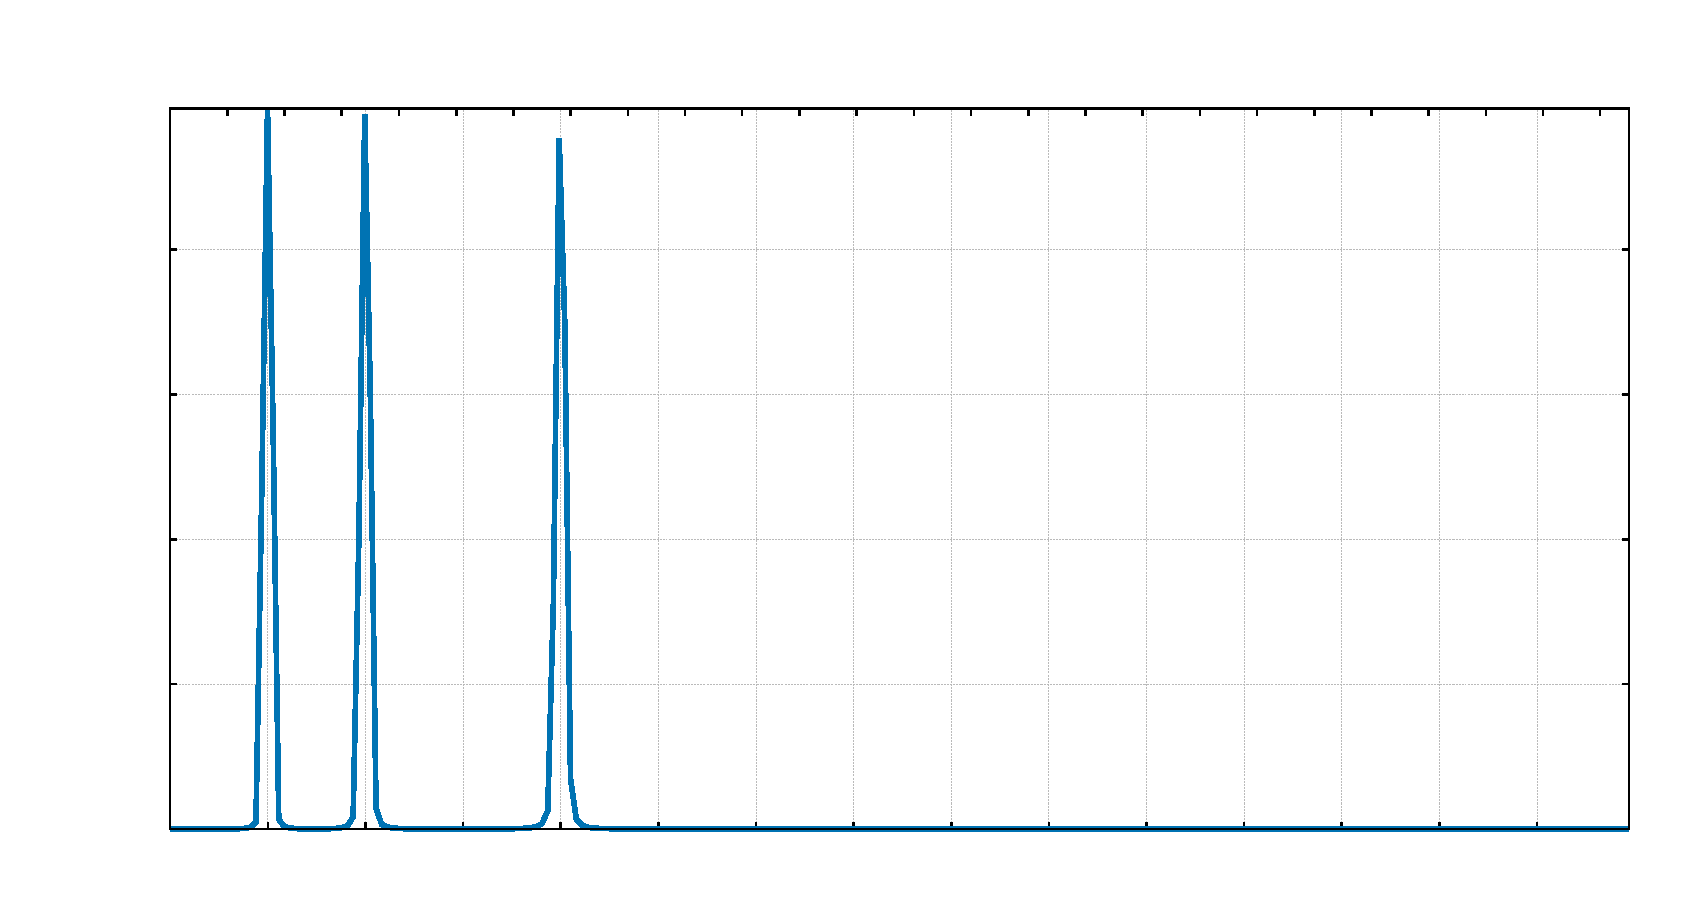
\includegraphics{res/plots/Q22B2SSB}}%
    \gplfronttext
  \end{picture}%
\endgroup
